% EnterpriseOS on AWS -- Cloud Computing project report (IEEE conference format)
% Compile on Overleaf (pdfLaTeX) or locally with: tectonic enterpriseos-aws-report.tex
\documentclass[conference]{IEEEtran}
\IEEEoverridecommandlockouts
\usepackage{cite}
\usepackage{amsmath}
\usepackage{graphicx}
\usepackage{booktabs}
\usepackage{array}
\usepackage{tabularx}
\usepackage{xcolor}
\usepackage{tikz}
\usetikzlibrary{arrows.meta,positioning,fit,backgrounds,shapes.geometric}
\usepackage[hidelinks]{hyperref}
\usepackage{url}

\definecolor{awsdark}{HTML}{232F3E}
\definecolor{impl}{HTML}{E8F1FF}
\definecolor{implborder}{HTML}{2B6CB0}
\definecolor{future}{HTML}{F2F2F2}
\definecolor{futureborder}{HTML}{8A8A8A}

\newcommand{\code}[1]{\texttt{\small #1}}

\begin{document}
\sloppy

\title{EnterpriseOS on AWS: A Cost-Safe Serverless and Event-Driven Cloud Architecture for Workforce Management}

\author{
\IEEEauthorblockN{Avik Khetarpal}
\IEEEauthorblockA{akhetarpal\_be24@thapar.edu}
\and
\IEEEauthorblockN{Humza Ali Choudhri}
\IEEEauthorblockA{hchoudhri\_be24@thapar.edu}
\and
\IEEEauthorblockN{Shashwat Tewari}
\IEEEauthorblockA{stewari\_be24@thapar.edu}
\and
\IEEEauthorblockA{\textit{Department of Computer Engineering, Thapar Institute of Engineering and Technology}\\
Cloud Computing ([Course Code]), Group [Group No.], Patiala, India}
}

\maketitle

\begin{abstract}
EnterpriseOS is a multi-tenant workforce-management application (employees, departments,
attendance, leave approvals, projects, tasks, notifications and audit activity) originally
built as a Node.js/Express modular monolith with PostgreSQL. This paper presents an
independent cloud edition that re-platforms the unchanged application onto Amazon Web
Services (AWS) under two hard constraints: zero personal expenditure, and the service and
identity restrictions of an AWS Academy sandbox. The application runs on AWS Lambda behind
an Amazon API Gateway HTTP API through a dependency-free loopback bridge; secrets are held
in AWS Systems Manager Parameter Store; leave decisions and task assignments are published as
versioned domain events to Amazon SQS and processed asynchronously by a second Lambda function
that fans out through Amazon SNS; CloudWatch provides structured logs and alarms; and the
entire stack is defined in one AWS SAM/CloudFormation template. The implementation is covered
by 56 passing automated tests (21 original and 35 new), passes template, script and workflow
linters, and reports no known dependency vulnerabilities. The sandbox's service list and
budget (US\$40, of which US\$0 used) were verified, giving a self-imposed credit cap of
US\$2.00 against an estimated US\$0.01--0.03 per demonstration session. At the time of
writing the stack is implemented and verified locally but not yet deployed; the paper
distinguishes these states explicitly.
\end{abstract}

\begin{IEEEkeywords}
Cloud computing, serverless, AWS Lambda, API Gateway, Amazon SQS, event-driven architecture,
infrastructure as code, cost optimisation, AWS Academy.
\end{IEEEkeywords}

\section{Introduction}
Cloud platforms promise elastic capacity, managed operations and pay-per-use pricing, but
students rarely get to apply them to a real application under realistic constraints. Our
Software Engineering project, EnterpriseOS~\cite{se-report}, provided such an application: a
browser-based workforce platform with role-based access control, tenant isolation and 21
automated tests, originally hosted on Vercel with a Neon PostgreSQL database.

This project asks a cloud-computing question about that system: \emph{how can an existing
web application be moved to AWS so that it demonstrates core cloud concepts (serverless
compute, managed messaging, secret management, observability, identity and access management
and infrastructure as code) without changing its business logic and without spending money?}
To protect the graded original, the work was carried out in a separate, private repository
with its own history; the original repository, deployment and database were not modified.

The contributions are: (i) a dependency-free adapter that runs the unchanged Express
application on Lambda; (ii) an asynchronous, retry-safe event pipeline with a dead-letter
queue; (iii) a parameterised, least-privilege SAM template that also works inside the AWS
Academy sandbox; (iv) a cost model and guard-rails that bound credit use; and (v) a
verification suite of 56 tests plus static checks.

\section{Problem Statement and Objectives}
\subsection{Constraints}
\begin{itemize}
\item \textbf{Zero personal cost.} No payment method may be attached and no paid plan used.
Free-tier eligibility is not assumed, because Academy accounts may not receive it.
\item \textbf{Academy restrictions.} The sandbox permits only two regions, forbids creating
IAM roles, users or identity providers, and permanently deletes all resources when a
session ends.
\item \textbf{Credit cap.} Academy credit use is limited to $\min(\text{US}\$3,\ 5\%$ of the
remaining budget$)$; if the budget cannot be read, the cap is US\$0.
\item \textbf{Preservation.} Existing routes, roles, responses and the local development
workflow must keep working.
\end{itemize}

\subsection{Objectives}
Run the application serverlessly with a managed HTTPS front door; keep all secrets out of
code, templates and logs; move slow side-effects to an asynchronous, observable pipeline;
describe the whole environment as code with a one-command teardown; and back every claim
about cost, security and deployment status with evidence.

\section{AWS Academy Environment Analysis}
The AWS Academy portal was inspected read-only after the student signed in. No separate
Learner Lab course was enrolled; the \emph{AWS Academy Cloud Developing 2.x Sandbox} was
identified as the deployment target. Its Readme~\cite{academy-readme} and status bar
provided the findings in Table~\ref{tab:env}.

\begin{table}[t]
\caption{Verified sandbox findings (25 Nov 2026)}
\label{tab:env}
\centering
\footnotesize
\begin{tabularx}{\columnwidth}{@{}lX@{}}
\toprule
Item & Finding \\
\midrule
Regions & us-east-1 and us-west-2 only \\
Budget & ``Used \$0 of \$40''; lags 8--12\,h (AWS Budgets) \\
Credit cap & $\min(\$3,\,5\%\times\$40)=\$2.00$ \\
Session & $\approx$3\,h timer; resources deleted at 0:00 \\
Over budget & Lab account disabled, resources lost \\
IAM & No new users, groups or roles; pre-created \code{LabRole} \\
Permitted & Lambda, API Gateway, SQS, SNS, CloudWatch, CloudFormation, Systems Manager, S3, CloudShell, DynamoDB, X-Ray, WAF \\
Not listed & AWS KMS (relevant to SecureString encryption) \\
\bottomrule
\end{tabularx}
\end{table}

Two findings shaped the design. Because IAM roles cannot be created, every function must be
able to run as \code{LabRole}, while a normal account should still get least-privilege
roles. Because resources are deleted when a session ends, deployment must be fast and
repeatable, which favours infrastructure as code over console configuration.

\section{Architecture}
\subsection{Overview}
Fig.~\ref{fig:arch} shows the target architecture. Dashed connectors denote components that
are implemented and tested but not yet deployed; grey components are designed only.

\begin{figure*}[t]
\centering
\resizebox{\textwidth}{!}{%
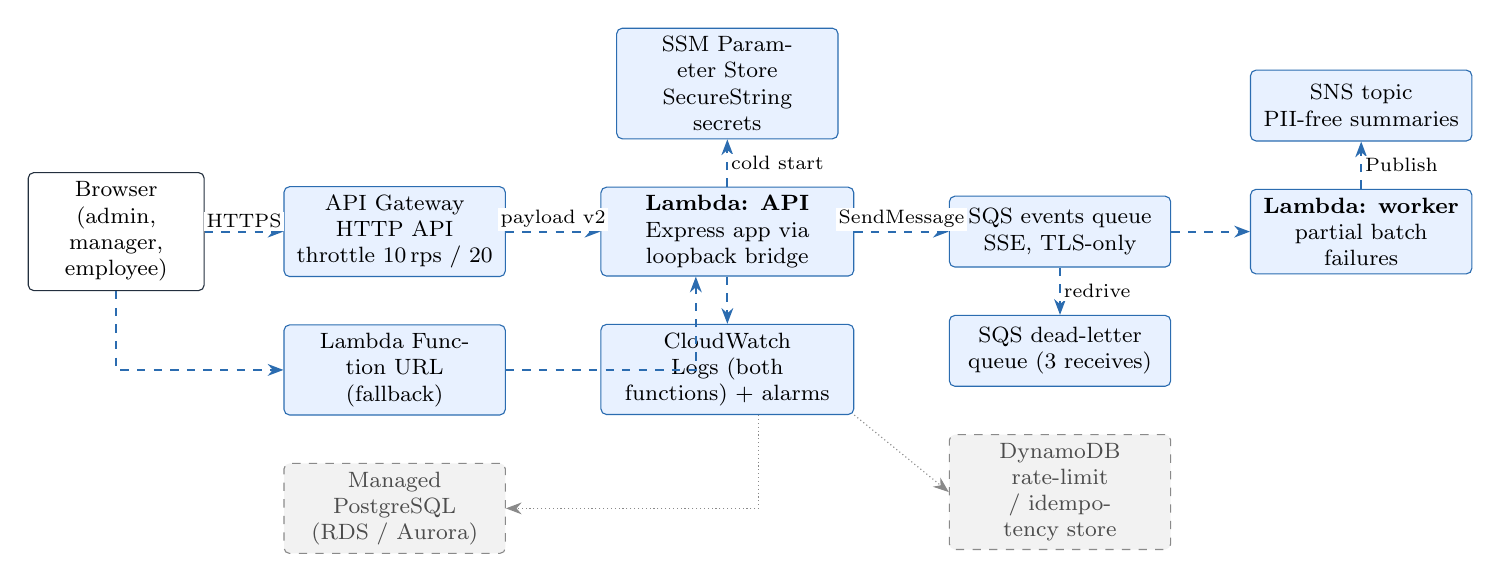
\begin{tikzpicture}[
  font=\footnotesize,
  box/.style={draw=implborder, fill=impl, rounded corners=2pt, align=center, minimum height=9mm, inner sep=3pt, text width=#1},
  box/.default=26mm,
  fut/.style={draw=futureborder, fill=future, dashed, rounded corners=2pt, align=center, minimum height=9mm, inner sep=3pt, text width=26mm, text=black!70},
  user/.style={draw=awsdark, fill=white, rounded corners=2pt, align=center, minimum height=9mm, text width=20mm},
  arr/.style={-{Stealth[length=2mm]}, dashed, draw=implborder, thick},
  farr/.style={-{Stealth[length=2mm]}, densely dotted, draw=futureborder},
  lbl/.style={font=\scriptsize, fill=white, inner sep=1pt}
]
\node[user] (u) {Browser\\(admin, manager,\\employee)};
\node[box, right=10mm of u] (gw) {API Gateway\\HTTP API\\throttle 10\,rps / 20};
\node[box, below=6mm of gw] (furl) {Lambda Function URL\\(fallback)};
\node[box=30mm, right=12mm of gw] (api) {\textbf{Lambda: API}\\Express app via\\loopback bridge};
\node[box, above=6mm of api] (ssm) {SSM Parameter Store\\SecureString secrets};
\node[box, right=12mm of api] (sqs) {SQS events queue\\SSE, TLS-only};
\node[box, below=6mm of sqs] (dlq) {SQS dead-letter\\queue (3 receives)};
\node[box, right=10mm of sqs] (wrk) {\textbf{Lambda: worker}\\partial batch\\failures};
\node[box, above=6mm of wrk] (sns) {SNS topic\\PII-free summaries};
\node[box=30mm, below=6mm of api] (cw) {CloudWatch Logs (both\\functions) + alarms};
\node[fut, below=6mm of furl] (pg) {Managed PostgreSQL\\(RDS / Aurora)};
\node[fut, below=6mm of dlq] (ddb) {DynamoDB rate-limit\\/ idempotency store};

\draw[arr] (u) -- node[lbl, above]{HTTPS} (gw);
\draw[arr] (u.south) |- (furl.west);
\draw[arr] (gw) -- node[lbl, above]{payload v2} (api);
\draw[arr] (furl.east) -| ([xshift=-4mm]api.south);
\draw[arr] (api) -- node[lbl, right]{cold start} (ssm);
\draw[arr] (api) -- node[lbl, above]{SendMessage} (sqs);
\draw[arr] (sqs) -- (wrk);
\draw[arr] (sqs) -- node[lbl, right]{redrive} (dlq);
\draw[arr] (wrk) -- node[lbl, right]{Publish} (sns);
\draw[arr] (api) -- (cw);
\draw[farr] ([xshift=4mm]cw.south) |- (pg.east);
\draw[farr] (cw.south east) -- (ddb.west);
\end{tikzpicture}%
}
\caption{Target AWS architecture of EnterpriseOS (\code{infrastructure/template.yaml}). Blue,
dashed: implemented and tested, not yet deployed. Grey, dotted: proposed future work. No
connection is drawn solid because nothing is deployed at the time of writing.}
\label{fig:arch}
\end{figure*}

\subsection{Service Selection}
Each service was chosen for a concrete need and for near-zero idle cost
(Table~\ref{tab:services}). Services that bill continuously (RDS, NAT gateways, load
balancers, EC2, Secrets Manager) were rejected, and an automated test fails if such resource
types appear in the template.

\begin{table}[t]
\caption{AWS services, purpose and status}
\label{tab:services}
\centering
\footnotesize
\begin{tabularx}{\columnwidth}{@{}l X l@{}}
\toprule
Service & Purpose in EnterpriseOS & Status \\
\midrule
Lambda (API) & Runs the unchanged Express app & Impl.\ locally \\
API Gateway HTTP & HTTPS, throttling, access logs & Impl.\ locally \\
Function URL & Fallback entry point & Impl.\ locally \\
SQS + DLQ & Durable event buffer, retries & Impl.\ locally \\
Lambda (worker) & Asynchronous event processing & Impl.\ locally \\
SNS & Fan-out of notifications/alarms & Impl.\ locally \\
SSM Param.\ Store & Encrypted secrets, no charge & Impl.\ locally \\
CloudWatch & JSON logs, 4 alarms, dashboard & Impl.\ locally \\
SAM/CloudFormation & Reproducible stack & Impl.\ locally \\
CloudFront + S3 & Edge static hosting & Designed \\
RDS / Aurora & Persistent shared database & Designed \\
GitHub OIDC role & Keyless CI deploys & Not available \\
\bottomrule
\end{tabularx}
\end{table}

\subsection{Request Flow}
A browser request reaches API Gateway, which applies stage throttling and forwards a
payload-format~2.0 event to the API function~\cite{aws-lambda}. On a cold start the handler (1) loads
allow-listed SecureStrings (\code{JWT\_SECRET}, optional \code{DATABASE\_URL}) from Parameter
Store before importing the application, because the application validates its secrets at
import time; (2) adds the API's own HTTPS origin, taken from the AWS-supplied
\code{requestContext.domainName}, to the CORS allow-list; (3) imports the unchanged Express
application; and (4) starts it on an ephemeral port bound to \code{127.0.0.1}. Each event is
then replayed as a genuine HTTP request on that loopback port and the response is converted
back (UTF-8 or base64 body, cookies separated). Every existing middleware (security headers,
CORS, body limits, JWT verification, forced password change, role checks and tenant-scoped SQL)
therefore runs exactly as it does locally.

\subsection{Event-Driven Processing}
After a manager decides a leave request or assigns a task, the API still writes the
notification and audit rows synchronously, preserving the original behaviour, and then
publishes a versioned event (\code{LEAVE\_DECIDED} or \code{TASK\_ASSIGNED}, carrying only
identifiers, type and status) to SQS. Publication failures are logged but never fail the
user's request. The worker receives batches of up to ten messages, validates each against
the event contract, writes a structured log entry and publishes a PII-free summary to SNS. It
returns \code{batchItemFailures} so that only failed messages are retried; after three receives
a message moves to the dead-letter queue, which triggers a CloudWatch alarm~\cite{aws-sqs}.
Delivery is at-least-once; each event carries a UUID for future idempotent consumers.

\subsection{Data Modes}
A managed database would add hourly charges and, for a VPC-attached Lambda, NAT or VPC
endpoint costs. The template therefore offers \code{DatabaseMode=ephemeral-demo} (the
application's existing in-memory engine, enabled only by an explicit flag) and
\code{DatabaseMode=postgresql} (a non-production connection string from Parameter Store).
Because each Lambda container holds its own in-memory data, demo seed records use
deterministic UUIDs, so all containers agree on users, tasks and leave requests and tokens
remain valid on any container. Writes are not shared between concurrent containers; this
limitation is documented rather than hidden.

\section{Implementation}
\subsection{Code Changes}
New code lives in \code{aws/lambda/} (API handler, HTTP bridge, Parameter Store loader, SQS
worker) and two small server modules (\code{events.js}, \code{logger.js}). Changes to existing
files were limited to a \code{/health} probe, request IDs and JSON access logging, event
publication after two existing workflows, an explicit opt-in for the demo database, and
deterministic seed IDs. No runtime dependency was added; the AWS SDK~v3 is provided by the
Lambda runtime and loaded lazily. The only new development dependency is a YAML parser used by
template tests.

\subsection{Infrastructure as Code}
A single SAM template~\cite{aws-sam} defines the functions, the HTTP API (or Function URL),
both queues and the queue policy, the topics, log groups with 7-day retention, alarms and an
optional dashboard. Parameters select the entry point, the data mode, the throttling limits and
the execution role: when \code{LambdaRoleArn} is empty, per-function inline policies grant
exact actions on exact ARNs; in the sandbox, \code{LabRole} is passed instead. The template
passes \code{cfn-lint} with no errors or warnings.

\subsection{Deployment Automation and CI/CD}
Shell scripts provide a read-only pre-flight check (region, caller identity, permissions,
secrets), secret creation that never prints values, a deployment that runs the tests,
packages and smoke-tests the artifact and requires typed confirmation of the change set, and a
cleanup that deletes the stack and then verifies that no function, queue or log group remains.
GitHub Actions run tests, dependency audits, a package smoke test, \code{cfn-lint}, ShellCheck
and a secret scan on every push~\cite{gh-actions}. Deployment and cleanup workflows are
manual-only and require a confirmation phrase; GitHub OIDC was designed but cannot be used
because the sandbox forbids creating identity providers.

\section{Security}
The original controls are preserved: bcrypt hashing, eight-hour JWTs~\cite{rfc7519}, role
middleware, tenant-scoped parameterised SQL, security headers and a login throttle. Cloud
controls were added following common API guidance~\cite{owasp} (Table~\ref{tab:security}). One cloud-specific risk deserved attention:
behind a proxy, every request appears to come from the same address, which would turn the
per-IP login throttle into a global one. The bridge therefore overwrites
\code{X-Forwarded-For} with the AWS-verified source IP and Express trusts exactly one
loopback hop; a test confirms that a forged header cannot bypass the throttle.

\begin{table}[t]
\caption{Cloud security controls}
\label{tab:security}
\centering
\footnotesize
\begin{tabularx}{\columnwidth}{@{}lX@{}}
\toprule
Risk & Control \\
\midrule
Secrets in code/env & SecureStrings loaded at cold start; tested absent from env vars \\
Over-privilege & Inline least-privilege policies; no wildcard actions (tested) \\
IP spoofing & \code{X-Forwarded-For} overwritten with AWS source IP \\
Data in transit/rest & TLS-only queue policy; SQS SSE; encrypted parameters \\
PII leakage & Events and SNS messages carry identifiers only \\
Denial of wallet & Stage throttling, alarms, short-lived stacks \\
Committed secrets & CI secret scan, canary-tested \\
\bottomrule
\end{tabularx}
\end{table}

The main accepted risk is that \code{LabRole} is much broader than the generated policies. It is
mitigated by short-lived stacks containing only synthetic data, and least privilege applies
automatically in any normal account.

\section{Cost Analysis}
Unit prices were taken from the AWS pricing pages for us-east-1~\cite{aws-lambda-pricing,
aws-apigw-pricing} without assuming any free tier. Table~\ref{tab:cost} summarises the
estimates. The only charges that continue while the stack is idle are CloudWatch alarms and
the SQS long-polling performed by Lambda's event-source mapping, together about US\$0.70 per
month. In the sandbox even these stop when the session ends. The worst case, sustained abuse
at the full throttle limit, is about US\$1.80 per day, which is why stacks are deleted after
each demonstration.

\begin{table}[t]
\caption{Estimated Academy credit consumption (no free tier)}
\label{tab:cost}
\centering
\footnotesize
\begin{tabularx}{\columnwidth}{@{}Xr@{}}
\toprule
Scenario & Estimate (US\$) \\
\midrule
One 3-hour demonstration session, then cleanup & 0.01--0.03 \\
Stack idle for 30 days (alarms + SQS polling) & $\approx$0.70 \\
Full-throttle abuse (10\,rps) for 24\,h & $\approx$1.80 \\
Verified credit cap for this project & 2.00 \\
Personal expenditure & 0.00 \\
\bottomrule
\end{tabularx}
\end{table}

\section{Testing and Evaluation}
The baseline suite (21 tests) passed before any change. After the work, 56 tests pass
(Table~\ref{tab:tests}). End-to-end tests invoke the real Lambda handler with
API Gateway-shaped events against the unchanged Express application, in the same
configuration as the cloud stack. The built deployment package (12.4\,MiB, production
dependencies only) is smoke-tested in isolation. Measured locally, a cold start including
demo seeding takes about 0.75\,s, excluding Lambda's own runtime initialisation, and a warm
request through the bridge adds about 1\,ms.

\begin{table}[t]
\caption{Verification results}
\label{tab:tests}
\centering
\footnotesize
\begin{tabularx}{\columnwidth}{@{}Xr@{}}
\toprule
Check & Result \\
\midrule
Original suites (auth, tenancy, bootstrap, time) & 21/21 \\
Lambda end-to-end (routes, CORS, throttle, events) & 11/11 \\
Bridge, Parameter Store, events, worker, logger & 12/12 \\
Data-mode guard, health probe, seed IDs & 4/4 \\
Template and workflow guard-rails & 8/8 \\
\textbf{Total} & \textbf{56/56} \\
\code{npm audit} (all / production) & 0 / 0 \\
\code{cfn-lint}, ShellCheck, actionlint & 0 findings \\
\bottomrule
\end{tabularx}
\end{table}

The new tests also exposed two pre-existing defects. The manager branches of the
leave-decision and task-status updates used correlated sub-queries that the in-memory engine
could not execute, so managers could not approve leave or move tasks in local mode. Both were
rewritten into semantically equivalent \code{IN} sub-queries and covered by regression tests.

\section{Deployment Status and Limitations}
\textbf{Deployment status:} at the time of writing, no AWS resource has been created; every
service in Table~\ref{tab:services} is \emph{implemented and verified locally}. The sandbox's
service list and budget have been verified and the deployment gate (pre-flight checks and a
cost checklist) is in place. Because the sandbox deletes resources when a session ends,
deployment is scheduled in the same session as the demonstration, and dated, redacted evidence
will be added to the repository. Other limitations: demo data is not shared between Lambda
containers; the login throttle is per container; KMS is not on the sandbox's service list,
so SecureString creation must be confirmed during the first session; and the PostgreSQL mode
was not exercised, because no non-production PostgreSQL server was available.

\section{Conclusion and Future Work}
EnterpriseOS was re-platformed onto a serverless, event-driven AWS architecture without
changing its business logic and with zero personal cost. The project shows that the core
cloud concepts (elastic compute, managed messaging with retries and dead-lettering, secret
management, least-privilege IAM, observability and infrastructure as code) can be
demonstrated within a constrained academic sandbox, provided that cost and deployment claims
are checked rather than assumed, in line with the cost-optimisation and security pillars of the AWS Well-Architected Framework~\cite{aws-wellarch}. Future work for a production deployment includes managed
PostgreSQL with RDS Proxy inside a VPC, CloudFront with AWS WAF and a custom domain, Amazon
Cognito or cookie-based sessions, a DynamoDB store for distributed rate limiting and
idempotency, AWS X-Ray tracing, and OIDC-based deployments with canary releases.

\begin{thebibliography}{00}
\bibitem{se-report} A. Khetarpal, H. A. Choudhri, and S. Tewari, ``Enterprise Workforce
Management System (EWMS): EnterpriseOS,'' Software Engineering (UCS503) project report,
Thapar Institute of Engineering and Technology, Nov. 2026.
\bibitem{academy-readme} Amazon Web Services, ``AWS Academy Cloud Developing 2.x -- Sandbox,''
lab Readme, accessed Nov. 25, 2026.
\bibitem{aws-lambda} Amazon Web Services, ``AWS Lambda Developer Guide.'' [Online]. Available:
\url{https://docs.aws.amazon.com/lambda/latest/dg/}
\bibitem{aws-sqs} Amazon Web Services, ``Amazon SQS Developer Guide: Dead-letter queues.''
[Online]. Available: \url{https://docs.aws.amazon.com/AWSSimpleQueueService/latest/SQSDeveloperGuide/}
\bibitem{aws-sam} Amazon Web Services, ``AWS Serverless Application Model Developer Guide.''
[Online]. Available: \url{https://docs.aws.amazon.com/serverless-application-model/}
\bibitem{aws-lambda-pricing} Amazon Web Services, ``AWS Lambda Pricing.'' [Online]. Available:
\url{https://aws.amazon.com/lambda/pricing/}
\bibitem{aws-apigw-pricing} Amazon Web Services, ``Amazon API Gateway Pricing.'' [Online].
Available: \url{https://aws.amazon.com/api-gateway/pricing/}
\bibitem{aws-wellarch} Amazon Web Services, ``AWS Well-Architected Framework.'' [Online].
Available: \url{https://docs.aws.amazon.com/wellarchitected/latest/framework/}
\bibitem{rfc7519} M. Jones, J. Bradley, and N. Sakimura, ``JSON Web Token (JWT),'' RFC 7519,
IETF, May 2015.
\bibitem{gh-actions} GitHub, ``GitHub Actions Documentation.'' [Online]. Available:
\url{https://docs.github.com/en/actions}
\bibitem{owasp} OWASP Foundation, ``REST Security Cheat Sheet.'' [Online]. Available:
\url{https://cheatsheetseries.owasp.org/cheatsheets/REST_Security_Cheat_Sheet.html}
\end{thebibliography}

\end{document}
